\section{Introduction des Solutions}
\label{introSolutions}
	Nous allons vous présenter les solutions que nous avons mis en place et les observations sur celles-ci. Le travail effectué dans Blue Banana (cf \ref{BlueBanana}, page \pageref{BlueBanana}) s'intéresse à une partie du jeu bien définie, qui est les déplacements entre les zones denses. Pour la première solutions, nous avons décidé de nous intéressé à une partie du jeu qui n'était pas encore étudié. Nous avons donc chercher comment améliorer le fonctionnent de notre solution dans les zones denses. 
\par Dans cette zone, les joueurs se déplacent de façon désordonnée et bougent la plupart du temps dans un secteur restreint. L'utilisation d'un cache est alors apparu comme une solution d'amélioration évidente. Un nœud va oublier des voisins dont il pourrait revoir dans un futur plus ou moins proche (en fonction de la mobilité dans le jeu), le cache va alors garder un certain nombre de ces nœuds dans l'éventualité où le nœud revienne sur ses pas (voir Schéma \ref{mouveDense}).Nous expliquerons les différentes solutions que nous avons testé pour le cache, et pourquoi celle que nous avons retenu fonctionnait le mieux.
	\vspace{5mm}
        \begin{figure}[!h]
        \centering
        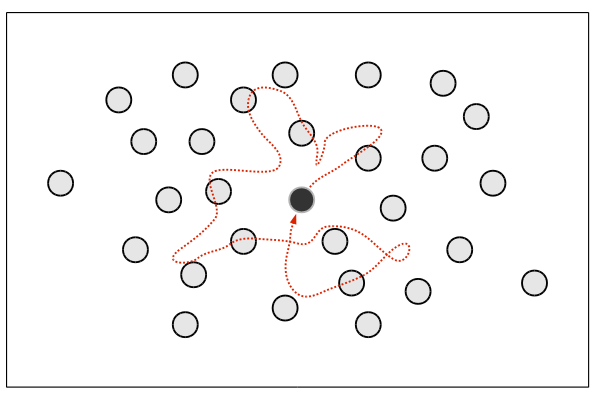
\includegraphics[scale=0.45]{./Ressources/Images/mouvementsZoneDense.png}\\
        \caption{Exemple d'une trajectoire d'un joueur dans une zone dense}
        \label{mouveDense}
        \end{figure}
\par Ensuite nous avons modifié le prefetching des données pour que celui-ci se fasse de manière plus fine, et que l'on puisse économiser des messages et améliorer sensiblement la cohérence de la topologie. Pour cette solution, nous passerons aussi en revu les différents techniques testées et celle retenue. 
